\documentclass[conference]{IEEEtran}

\usepackage{cite}
\usepackage{amsmath,amssymb}
\usepackage{booktabs}
\usepackage{graphicx}
\usepackage{url}
\usepackage{algorithm}
\usepackage{algorithmic}
\usepackage[T1]{fontenc}
\usepackage[utf8]{inputenc}

\def\BibTeX{{\rm B\kern-.05em{\sc i\kern-.025em b}\kern-.08em T\kern-.1667em\lower.7ex\hbox{E}\kern-.125emX}}

\begin{document}

\title{Which Way Does Fairness Go? The Selection Rate Predicts\\
Whether an Attribute-Blind Constraint Gives or Takes}

\author{\IEEEauthorblockN{Dheirav}
\IEEEauthorblockA{\textit{Responsible AI} \\
\textit{Algorithmic Bias Mitigation}\\
\texttt{dheirav2005@gmail.com}}}

\maketitle

\begin{abstract}
A group-fairness constraint requires two groups' selection rates to be close, but it does not
say how the gap should close: the disadvantaged group can be lifted, or the advantaged group
can be pulled down. Both outcomes satisfy the constraint, and the metric that certifies it
reports the same number in each case, which means a deployment team cannot tell from its own
dashboard which of the two it is about to cause. We show that the direction is predictable in
advance from a quantity every deploying organisation already has: the rate at which its
current model says yes, read against that population's crossover. Across 57 independent
populations covering six decision domains and seven data sources, an attribute-blind parity
constraint withdraws favourable decisions when the baseline selection rate sits below a
crossover, and extends them when it sits above; on UCI Adult six in-processing methods each
shrink the pool by 7.9--22.1\%, while on mortgage lending the identical constraint grows it.
The crossover's location is population-specific --- located values span 0.28 to 0.65, and
the fixed 0.54 prior is a fallible substitute for measuring one's own: sealed at
\textbf{9 of 10} on one cohort of never-measured populations (best constant 6), 5 of 10
post-hoc on a second cohort of larger states, every miss agreeing with that population's
own crossover. The sealed cohort's rule, populations and pass mark were committed to
version control before any run; an earlier sealed attempt that carried an in-sample
refinement \textbf{failed at four of eight}, and we report both outcomes because the
difference between them is what a sealed test exists to expose. A caution that generalises
beyond this paper: four 2022 populations initially appeared to \emph{invert} the
relationship, and diagnosis traced this substantially to the fixed nominal \$50{,}000
label sliding down an inflated income distribution --- a fixed nominal outcome definition
is a different task each year, so labels should be real-anchored and any deployment should
measure its own current data rather than transport results across vintages. The relationship survives
a change in how the rate is varied, a twenty-five-fold range of constraint tolerance, a
boosted-tree learner and a protected attribute swapped from sex to race, but it disappears
under post-processing ($r = -0.024$ against $+0.585$), which reads the protected attribute at
decision time. That boundary is where contemporaneous theory says the direction stops being
distributional and becomes determined, and the theory's prediction for that regime holds in
27 of 27 populations, nine pre-registered. The practical outcome is a procedure: when the
deployed model's viable operating band is wide enough --- which the procedure itself checks
first --- a team can locate its own crossover by sweeping that model's threshold, using no
new data.
\end{abstract}

\begin{IEEEkeywords}
algorithmic fairness, levelling down, demographic parity, in-processing, selection rate,
disparate impact
\end{IEEEkeywords}

\section{Introduction}

A fairness constraint says that two groups' rates should be close, but it does not say how
that closeness should be reached. The gap can close because the disadvantaged group is
lifted, or because the advantaged group is pulled down, and while both directions satisfy
the constraint, they are morally very different outcomes on most --- though, we note, not
all --- accounts of what the constraint is for; at minimum, anyone imposing one deserves
to know which they are getting.

This ambiguity is already well established. Mittelstadt \emph{et al.} \cite{mittelstadt2023}
made levelling down the centre of a well-known critique; Maheshwari \emph{et al.}
\cite{maheshwari2023} observe that it ``often goes unnoticed in the overall performance of
the model''; and Ferry \emph{et al.} \cite{ferry2023} built an auditing framework precisely
because an aggregate score reports neither how many people were affected nor in which
direction. We take all of that as given.

What the literature leaves open is the question a deploying team actually faces:
\textbf{when} does each direction happen? A team cannot act on ``this sometimes occurs'',
but it can act on a rule that says which way its own system will move before it moves, which
is what this paper provides and tests.

\subsection{Scope, stated first}

This is a paper about \textbf{attribute-blind in-processing} constraints, meaning the regime
in which the protected attribute is unavailable at decision time. This is the regime most
deployed systems occupy: in the United States, per-group decision thresholds face direct
disparate-treatment exposure (\emph{Ricci v.\ DeStefano} \cite{ricci2009}; in credit, ECOA
and Regulation B prohibit attribute-based terms outright), and commentators read the
doctrine the same way \cite{barocas2016,corbett2017}. Two honest qualifications: the
barrier is jurisdiction-specific (in the EU it runs through data-protection law rather than
a per-group-threshold ban), and even \emph{training-time} use of the attribute --- which
every in-processing method here involves --- is legally unsettled in the US, so we motivate
the regime as the one systems occupy, not as one the law cleanly compels. Under
post-processing, which does read the attribute, the effect we report disappears
(Section~\ref{sec:regime}). We treat this not as a weakness of the finding but as the
boundary the theory draws, and we verify it from both sides.

\subsection{Contributions}

\begin{enumerate}
\item \textbf{An empirical characterisation of a conditionality that theory predicts.}
Contemporaneous theory \cite{backfire2026} establishes that in the attribute-blind regime the
direction is distribution-dependent. It contains no experiments and its conditions are ordering
relations on score regions rather than measurable quantities. We supply the measurement across
57 populations and six domains, and find that under our probe estimator its stated
conditions --- which are \emph{sufficient, not necessary} --- could not be certified on any
of 26 real arms (Section~\ref{sec:regime}), while a relaxed form of the same ordering
agrees with the measured direction on 24 of 26 and correlates with our predictor at
$r = +0.935$: the selection rate operationalizes the theory's quantity. The direction rule
itself is \emph{sealed}: committed before ten populations this work had never measured, it
scored 9 of 10 against a best constant of 6 (Section~\ref{sec:resealed}); on a second,
post-hoc cohort of larger states the fixed prior scored 5 of 10, each miss agreeing with
that population's own measured crossover.

\item \textbf{Two predictive claims, distinguished by what they require.} The paper contains
a \emph{sweep-conditional} claim --- run the audit on your own data and, where the response
is monotone, the rate against your own measured crossover predicts direction --- and a
weaker \emph{transported-prior} claim, the only one testable before any measurement, whose
record is the sealed 9 of 10 followed by 5 of 10. Varying the selection rate by moving a
label threshold cannot alone distinguish ``the rate predicts'' from ``task difficulty
does''; holding the task fixed and moving only the decision rule separates them across the
mid-range, and we say \emph{predicts}, never \emph{causes}: no pooled slope transfers
across populations (Section~\ref{sec:boundaries}).

\item \textbf{A procedure, not an observation.} The same design lets a practitioner locate
their own crossover on a deployed model. Four independent estimates of the mortgage crossover
agree.

\item \textbf{Boundaries stated explicitly rather than left for review to find}, including a
computable test for when the procedure cannot be used at all.
\end{enumerate}

\section{Related Work}

\textbf{Whether levelling down is universal.} A 2026 theory paper \cite{backfire2026} proves in
a population-level Bayes framework that the answer depends on the deployment regime. Where the
protected attribute is available at decision time, fairness ``necessarily (weakly) improves
outcomes for the disadvantaged group and (weakly) worsens outcomes for the advantaged group''.
Where it is not --- the attribute-blind regime, which is ours --- ``the impact of fairness is
distribution-dependent: fairness can benefit or harm either group $\ldots$ leading to either
leveling up or leveling down.'' \textbf{We therefore do not claim the conditionality itself.}

\textbf{Levelling down, and the remedy.} Mittelstadt \emph{et al.} \cite{mittelstadt2023} argue
that fairness interventions frequently equalise by degrading the better-off group, and
\emph{also propose the remedy}: minimum rate constraints requiring ``that every group has, at
least, a minimal selection rate, precision, or recall''. We claim neither the observation nor
the remedy as novel. Our contribution relative to that work is narrow and checkable: a scope
condition they do not have; in-processing rather than post-processing, so no model reads the
attribute when predicting; a population-level floor stacked \emph{with} parity rather than a
per-group floor replacing it; and held-out replication where they report training-set results.

\textbf{Auditing individual impact.} Ferry \emph{et al.} \cite{ferry2023} propose a framework
whose first three dimensions are impact size, change direction and decision rates. That is the
decomposition we use throughout, and we claim no part of it. What we add is what those axes
report at scale: the change-direction dimension is not a property of the method being audited
but of the population it is applied to.

\textbf{The shape of the optimal fair classifier.} Corbett-Davies \emph{et al.}
\cite{corbett2017} show that for several fairness definitions the optimal constrained
classifier takes the form of group-specific risk thresholds. This gives a \emph{bound} rather
than another baseline: it predicts that levelling down is not an artifact of the reduction's
search, because the optimal constrained classifier withdraws in the same way.

\textbf{Remedies that avoid harm.} Minimax group fairness \cite{diana2021} minimises the worst
group's error rather than equalising anything, and is the natural alternative to a parity
constraint for a team whose concern is harm rather than equality. We benchmark against it
rather than only against the unconstrained reduction.

\textbf{The selection-rate axis.} The nearest prior work is Goethals \emph{et al.}
\cite{goethals2024}, which studies the cost of fairness as a function of available budget and
reports that ``the level of available resources significantly influences this cost, a factor
overlooked in previous evaluations''. The difference is structural: in their setting positive
decisions are a fixed resource, so the total is constant by construction and the directional
effect we measure cannot arise.

\textbf{Fairness gerrymandering and dataset monoculture.} Kearns \emph{et al.}
\cite{kearns2018} show constraints on marginal groups can be satisfied while subgroups are
badly treated. Ding \emph{et al.} \cite{ding2021} argue the field should stop drawing
conclusions from UCI Adult and supply ACS-derived replacements. Notably they also
\emph{build the knob this paper turns}: the \$50{,}000 threshold ``was chosen so that this
dataset can serve as a replacement to UCI Adult, but we also offer datasets with other income
cutoffs''. They do not connect it to the direction of a fairness intervention --- their text
contains no occurrence of ``selection rate'', ``acceptance rate'' or ``leveling down'' --- so
the instrument existed and the question was not asked of it. We replicate across their
populations and then find that is \emph{not sufficient}, because they share one survey
instrument.

\section{Setup and Method}

\textbf{Data.} Fifty-seven independent populations across seven data sources: UCI Adult
(45{,}222 rows); ACS Income \cite{ding2021} across forty US states, ten further
state-years (2014, 2019 and 2022) and two protected attributes; HMDA mortgage records for two states, by race and sex and split by loan purpose;
COMPAS \cite{propublica2016} (5{,}278 rows on the race arm after ProPublica's documented
filter); LSAC bar passage (20{,}798 rows); the Dutch national census of 2001 (60{,}420
rows); and Taiwanese credit-card default records of 2005 (30{,}000 rows). A
\emph{population} here is one such unit --- a state, cohort or census --- and
\emph{independent} means disjoint person samples: no person appears in two of them, and
arms within a population share people, so however many arms a population contributes, it
is counted once (Table~\ref{tab:accounting}); the seven data sources remain the honest
count of independent \emph{instruments}. Three survey-methodology conventions are
deliberate and inherited from the folktables benchmark \cite{ding2021}: ACS person records
are used \emph{unweighted} (no \texttt{PERWT}), incomes are nominal \texttt{PINCP} without
the \texttt{ADJINC} adjustment, and household clustering is not modelled, so every
``selection rate'' here is a property of the unweighted sample rather than a
design-consistent state estimate, and seed-resampled intervals are anti-conservative. A
weighted re-analysis is reported as ongoing work.

COMPAS, LSAC and the Dutch census were added to leave the sources the finding was formed
in. The Dutch census
carries a between-group gap of 0.298, roughly twice Adult's, making it the test of the standard
alternative explanation. LSAC was chosen because bar passage is naturally generous (base rate
0.890).

\textbf{Convention.} $y = 1$ is always the favourable outcome. This required inverting COMPAS's
recorded target, which encodes recidivism, and declaring \emph{Female} the advantaged group on
its sex arm, since women in that cohort reoffend less. Both are enforced by automated checks,
because either error produces every directional result sign-inverted without raising.

\textbf{Mitigation.} \texttt{ExponentiatedGradient} \cite{agarwal2018} at $\varepsilon = 0.01$
unless stated. No model reads the protected attribute at prediction time except where
post-processing is explicitly under test.

\textbf{Exclusion rules.} An arm is discarded if the baseline demographic-parity gap is below
0.05, or if the baseline classifier's accuracy falls below $\max(p, 1-p)$ --- the accuracy of
always predicting the more common label. The second rule matters more than it sounds
(Section~\ref{sec:failures}). Provenance, because exclusion rules can select on outcomes:
both rules were developed \emph{during} the exploratory phase, in response to failures the
ledger records, so retained-arm correlations from that phase are conditioned on
in-sample-tuned filters and the sensitivity table reports the dependence; every sealed test
from the re-seal onward carried both rules frozen in its pre-committed protocol.

\textbf{Accounting.} Table~\ref{tab:accounting} states which populations enter which
analysis, because three counts in this project's own history turned out to be arm counts
masquerading as population counts, and a reader should not have to reconstruct the
denominators.

\begin{table}[t]
\caption{Which populations enter which analysis. An \emph{arm} is one population under one
configuration; populations are counted once however many arms they contribute.}
\label{tab:accounting}
\centering
\footnotesize
\setlength{\tabcolsep}{3pt}
\begin{tabular}{@{}ll@{}}
\toprule
\textbf{Analysis} & \textbf{Populations (arms)} \\
\midrule
Ablation; who pays & Adult (6 methods $\times$ 5 seeds) \\
Rate--people divergence & 10 pops.\ (19 arms, 2 attributes) \\
Label route (income cutoffs) & AL sex; AL, MS, OR, UT race (4 each) \\
Natural transition & HMDA MS+LA (5 loan purposes) \\
Threshold route, dense sweeps & Dutch, SC, COMPAS, AL, KY (12 pts.) \\
Tolerance, $25\times$ range & AL, CT, KY, OR, SC \\
Boosted trees & the same five states \\
Intersectional & Adult + 10 populations \\
Post-processing regime & 17 populations ($r=-0.024$) \\
Attribute-aware direction & 27 of 27, of which 9 pre-registered \\
Relaxed $\zeta$ ordering & 26 arms from 15 populations \\
Crossover intervals & 4 non-lending + 3 lending estimates \\
Sealed test 1 (failed) & 8 scored + Taiwan, all fresh \\
Re-seal (holds) & 10 fresh ACS states \\
Residual campaign (underpow.) & 10 fresh states (76 arms) \\
Sealed magnitude (failed) & NY + TX (16 arms) \\
Cross-year shape seal (failed) & 8 fresh state-years (70 runs) \\
Attr.-independence seal (failed) & 6 race arms (48 runs) \\
Selection-rate floor & 10 pops.\ (19 arms) \\
\bottomrule
\end{tabular}
\end{table}

\section{Parity Is Reached by Withdrawal --- in Some Populations}

\begin{table}[t]
\caption{Six in-processing methods on UCI Adult, five seeds. Every one reaches parity, and
every one shrinks the pool.}
\label{tab:ablation}
\centering
\small
\begin{tabular}{@{}lccccr@{}}
\toprule
\textbf{Method} & \textbf{Acc.} & \textbf{DP} & \textbf{EO} & \textbf{DI} &
\textbf{$\Delta$pool} \\
\midrule
Unconstrained & 0.847 & 0.186 & 0.095 & 0.300 & --- \\
\midrule
ExpGrad (DP) & 0.828 & \textbf{0.018} & 0.280 & 0.895 & $-20.5\%$ \\
GridSearch (DP) & 0.827 & \textbf{0.015} & 0.304 & 0.986 & $-22.1\%$ \\
Adversarial deb. & 0.826 & 0.020 & 0.250 & 0.889 & $-14.8\%$ \\
Prejudice remover & 0.837 & 0.065 & 0.188 & 0.686 & $-10.2\%$ \\
ExpGrad (EO) & 0.836 & 0.107 & \textbf{0.032} & 0.521 & $-7.9\%$ \\
\bottomrule
\end{tabular}
\end{table}

Table~\ref{tab:ablation} gives the ablation. Every method reaches its target: demographic
parity falls from 0.186 to as little as 0.015 for under two accuracy points, and this holds
on a linear model and on an adversarial one alike. The mitigation itself works, which is why
we treat it as background rather than as a contribution.

What changes alongside is the part the metric does not report: \textbf{every one of these
methods shrinks the pool}, by 7.9\% to 22.1\%, and not one of them closes the gap primarily
by extending decisions to the disadvantaged group. Eighteen of nineteen survey arms show the
same pattern, which suggests this is a property of the populations rather than of any one
method.

\subsection{Rates understate what is happening to people}

\begin{table}[t]
\caption{Who pays, UCI Adult. The rate-level view and the people-level view of the same
intervention disagree systematically.}
\label{tab:whopays}
\centering
\small
\begin{tabular}{@{}lccc@{}}
\toprule
\textbf{Method} & \textbf{Share (rates)} & \textbf{Share (people)} & \textbf{Exchange} \\
\midrule
ExpGrad (DP) & 0.575 & \textbf{0.742} & 2.68 \\
GridSearch (DP) & 0.575 & \textbf{0.743} & 2.69 \\
Adversarial deb. & 0.508 & \textbf{0.700} & 1.96 \\
Prejudice remover & 0.498 & \textbf{0.673} & 2.04 \\
ExpGrad (EO) & 0.531 & \textbf{0.660} & 1.92 \\
\bottomrule
\end{tabular}
\end{table}

The decomposition of \cite{ferry2023} splits the closed gap into the part paid by the
advantaged group losing ground and the part gained by the disadvantaged group. Measured in
\emph{rates}, that split is close to even --- 0.50 to 0.58 of the closure comes from
withdrawal (Table~\ref{tab:whopays}).

Measured in \emph{people} the split is not even. Between 0.66 and 0.74 of the individuals
whose decision changed are members of the advantaged group losing a favourable one. The
reason the two views disagree is that equal-looking rate changes fall on groups of unequal
size, so the rate-level view --- which is what a fairness dashboard reports --- understates
the burden counted in individuals, and it does so in every method tested. The divergence
between the two views is itself predictable from a cross-flow diagnostic, at $r = +0.885$
across populations.

The \textbf{exchange rate} shows the same thing without needing a share: ExpGrad under
demographic parity destroys 2.68 favourable decisions for every one it creates.

\textbf{The normative baseline, stated as the convention it is.} Throughout, ``withdrawal'',
``who pays'' and the exchange rate are counterfactual-comparative quantities measured
against the \emph{unconstrained model's} allocation --- a baseline with no privileged moral
standing, since the constraint exists precisely because that allocation is suspect. On a
claims-based view \cite{broome1990}, withdrawing an approval that answered to no legitimate
claim wrongs no one; a positive classification is also not automatically a benefit
(extension in lending can be predatory inclusion). The exchange rate is therefore an
unweighted descriptive count, not a welfare ledger: a reader with prioritarian weights on
the disadvantaged group's gains may score a rate above 1.0 as net-good, and the
group-conditional flows the tables report make such weighted readings computable. What the
accounting establishes is narrower and metric-relative: the certifying number cannot tell
these outcomes apart, whatever one's weights.

On HMDA mortgage data, however, the direction reverses. The identical constraint \emph{grows}
the pool by 4.3\%, at an exchange rate of 0.50 --- two favourable decisions created for every
one destroyed. What makes this worth noticing is that the parity metric cannot see the
difference: it reports 0.018 on the population that destroyed a fifth of its favourable
decisions, and 0.010 on the one that created more than it destroyed.

\section{What Predicts the Direction}

\begin{figure*}[t]
\centering
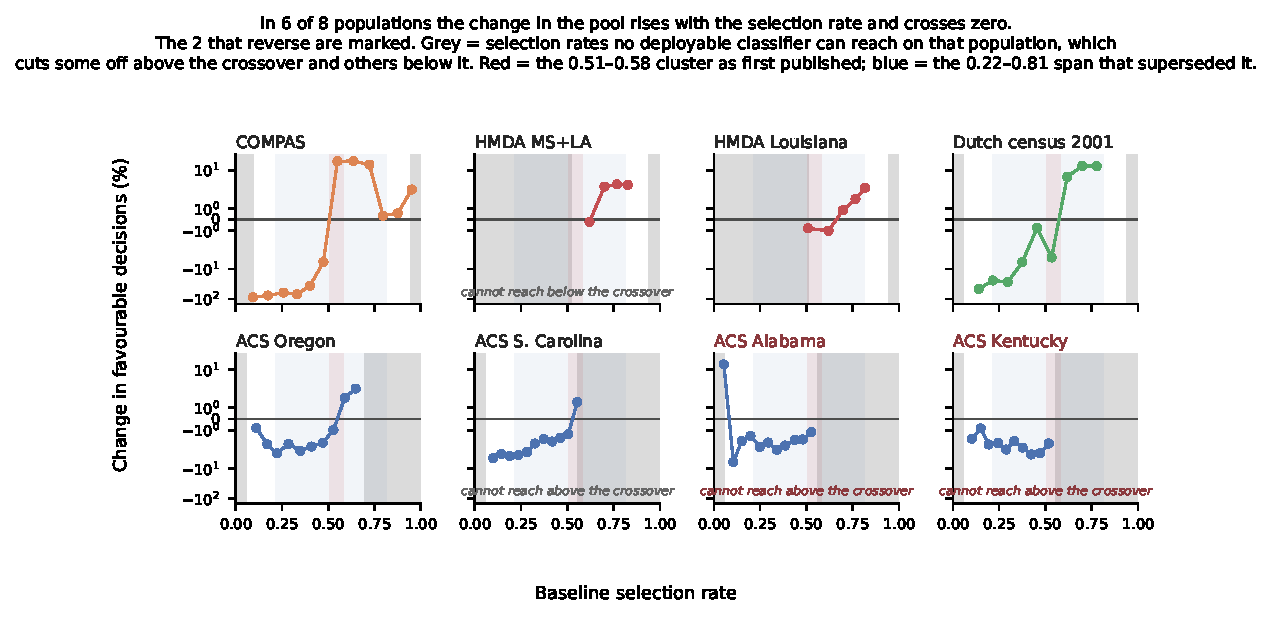
\includegraphics[width=\textwidth]{fig-crossover.pdf}
\caption{Every retained arm from every densely swept population. Within a population the
change in the pool rises with the baseline selection rate and crosses zero; the two that
reverse are marked, and both are sweeps whose viable band confines them below the crossover.
Panels are deliberately \emph{not} pooled: across populations a single slope reaches only
$r=+0.487$ and fails its pre-registered bar, so one scatter would assert a common curve the
data rejects. Vertical band: the 0.511--0.576 cluster of point estimates from
Table~\ref{tab:crossover}; carrying that table's bootstrap intervals widens it to roughly
0.43--0.58.}
\label{fig:crossover}
\end{figure*}


\subsection{A single-factor design}

ACS Income's label is ``earns more than \$50{,}000'', and that threshold is a benchmark
convention rather than a fact about the world, which makes it a knob we can turn. Moving it
on one fixed state varies the selection rate while the population, instrument, feature set,
group ratio and proxy structure all stay fixed. The change in the pool rises with the
baseline selection rate at $r = +0.801$ over four arms --- too few points for formal
inference, and reported as descriptive; a partial correlation on four points has one
degree of freedom and is omitted as uninformative. The sign flip is the substantive
observation: 22 decisions are destroyed per one created at a rate of 0.03, compared with
0.75 at 0.89.

\subsection{The transition appears without being manufactured}

The same transition also appears where nothing is manipulated at all. Pooling two states
across five real loan products, home improvement at a selection rate of 0.555 levels
\emph{down} ($-1.57\%$) while refinancing at 0.871 levels \emph{up} ($+2.95\%$), with
$r = +0.803$ and Spearman $\rho = +0.900$. This means a bank running one constraint across
its loan book would take opportunities away in one product while handing them out in
another, and its fairness report would show success in both.

\subsection{It is the rate, not the difficulty of the task}
\label{sec:tworoutes-note}

\begin{figure*}[t]
\centering
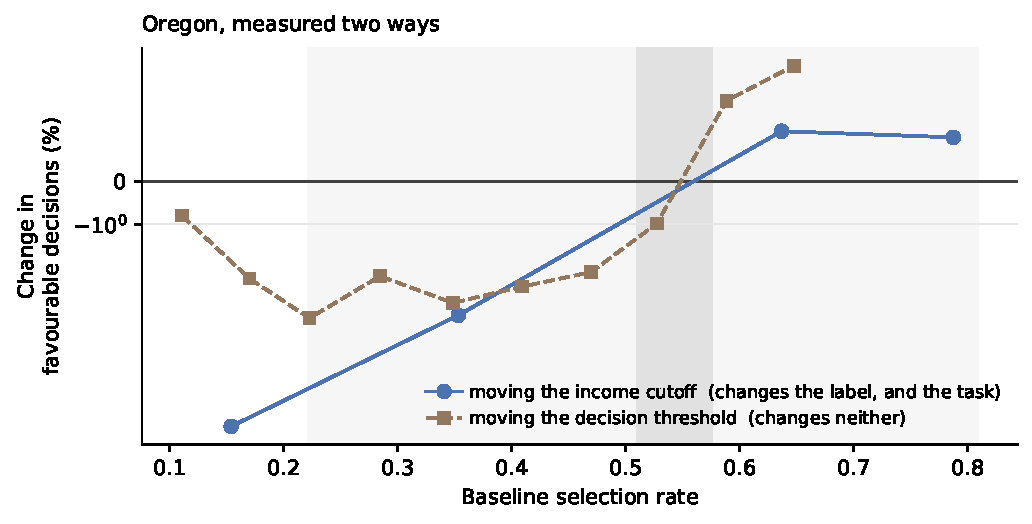
\includegraphics[width=0.86\textwidth]{fig-two-routes.pdf}
\caption{The design that separates the selection rate from the difficulty of the task. Moving
the income cutoff changes the label, and therefore how hard the problem is; moving the decision
threshold changes neither, only where the fitted model draws its line. Both routes cross zero
inside the same band. If difficulty were doing the work, the second curve would not reproduce
the first.}
\label{fig:tworoutes}
\end{figure*}


The design above moves the \emph{label}. ``Earns over \$100{,}000'' is not a rarer version of
``earns over \$20{,}000''; it is a harder problem. That design therefore cannot separate two
explanations which predict everything observed so far.

We separate them by holding the task completely fixed --- same rows, features, groups and
\emph{fitted scores} --- and moving only where the model draws its line. The relationship
reproduces, and so does the crossover's location: on Oregon the two routes give 0.362--0.653
and 0.353--0.637. \textbf{Task difficulty is not doing the work.}

With twelve points chosen from each population's viable band, the relationship holds on the
Dutch census ($+0.946$), South Carolina ($+0.905$) and COMPAS ($+0.844$). Alabama and Kentucky
return \emph{negative} values on eleven and ten arms; their viable bands top out at 0.566 and
0.561, at or below every crossover measured, so both sweeps lie almost entirely on one side of
the transition. \textbf{We therefore claim the relationship across the crossover and withdraw
any claim that it holds within the low-rate region alone.}

\subsection{Five domains, and the group-gap alternative}

\begin{table}[t]
\caption{The relationship across instruments. Each $r$ is computed within one population of
that instrument, over the retained arms counted in the last column --- not pooled across the
instrument, for the reason Fig.~\ref{fig:crossover} does not pool.}
\label{tab:domains}
\centering
\footnotesize
\setlength{\tabcolsep}{4pt}
\begin{tabular}{@{}lllcc@{}}
\toprule
\textbf{Instrument} & \textbf{Domain} & \textbf{Population} & \textbf{$r$} & \textbf{Arms} \\
\midrule
ACS Income & income & Alabama & $+0.801$ & 4 \\
HMDA & mortgages & MS+LA pooled & $+0.858$ & 4 \\
COMPAS & crim. justice & race arm & $+0.870$ & 5 \\
Dutch census & occupation & sex arm & $+0.915$ & 6 \\
LSAC & legal educ. & --- & unsweepable & --- \\
\bottomrule
\end{tabular}
\end{table}

Fig.~\ref{fig:crossover} shows every arm, and Table~\ref{tab:domains} the summary. The pre-registered alternative --- ``this is a
property of income prediction and American mortgage lending'', requiring $|r| < 0.30$ --- loses
on both new instruments.

The oldest competing account is that the \emph{gap between groups} drives the direction. The
Dutch census has a gap of 0.298, roughly twice Adult's, making it the population where that
explanation should win. It gives $r = +0.915$ across all six arms, none excluded.

\subsection{Robustness}

\begin{table}[t]
\caption{What each manipulation preserves}
\label{tab:robust}
\centering
\small
\begin{tabular}{@{}lll@{}}
\toprule
\textbf{Manipulation} & \textbf{Direction} & \textbf{Magnitude} \\
\midrule
Route to the rate & unchanged & differs $3\times$ \\
Tolerance, $25\times$ range & unchanged & differs $4\times$ \\
Boosted trees (5/5 pops.) & unchanged & differs $3\times$ \\
Attribute, sex $\rightarrow$ race & unchanged & --- \\
Criterion $\rightarrow$ equalized odds & weaker, unevenly & differs $8\times$ \\
Optimiser $\rightarrow$ post-proc. & \textbf{vanishes} & --- \\
\bottomrule
\end{tabular}
\end{table}

Table~\ref{tab:robust} summarises. \textbf{Within a population, and in the attribute-blind regime, the selection rate
predicts which way and orders how much. Neither transfers between populations}: the signed distance from a
population's own crossover gives $\rho$ of $+0.96$, $+0.95$ and $+0.78$ in three of four
populations, but a pooled slope reaches only $r = +0.487$ against a pre-registered $+0.70$ bar.

\section{A Constraint on One Attribute Leaves Subgroups Behind}
\label{sec:intersectional}

\begin{table}[t]
\caption{UCI Adult. Constraining sex to 0.020 leaves the worst \emph{Sex}$\times$\emph{Race}
subgroup gap at 0.178 --- nine times larger --- and moves which subgroup is worst off.}
\label{tab:intersectional}
\centering
\footnotesize
\setlength{\tabcolsep}{4pt}
\begin{tabular}{@{}lccl@{}}
\toprule
\textbf{Arm} & \textbf{Sex} & \textbf{Subgroup} & \textbf{Worst off} \\
\midrule
Unconstrained & 0.190 & 0.315 & F$\times$Black \\
Constrained on sex & \textbf{0.020} & \textbf{0.178} & M$\times$Black \\
Constrained on both & 0.016 & 0.048 & F$\times$White \\
\bottomrule
\end{tabular}
\end{table}

A constraint is imposed on the attribute someone chose to name. Kearns \emph{et al.}
\cite{kearns2018} showed that marginal constraints can be satisfied while structured subgroups
are badly treated. Table~\ref{tab:intersectional} is that failure mode measured on Adult.

Constraining sex drives its gap from 0.190 to 0.020 --- a success by the certifying metric.
The worst \emph{Sex}$\times$\emph{Race} subgroup gap falls only from 0.315 to 0.178, which is
\textbf{nine times} the gap that was constrained. The subgroup carrying the residual also
\emph{changes}, from Female~$\times$~Black to Male~$\times$~Black, so an auditor tracking the
originally worst-off cell would see improvement while a different cell absorbed the cost.

This replicates across populations and is more severe than Adult suggests: 13.2$\times$ in
Mississippi. It is bounded, however, by how large the minority is --- the effect scales with
minority share at $r = -0.671$, and does not appear at all below a threshold. We present this
as an empirical replication of \cite{kearns2018} and \cite{maheshwari2023} with a boundary
attached, not as a new observation.

\textbf{A measurement hazard worth naming.} Roughly five subgroups per population are too small
to support any estimate. A rate with an empty denominator must return undefined rather than
zero, or an unmeasurable subgroup masquerades as a perfectly fair one --- which is the failure
this analysis is most likely to produce and hardest to notice.

\section{The Regime Boundary}
\label{sec:regime}

The last row of Table~\ref{tab:robust} looks like a failure of robustness, but we read it
differently, because it falls exactly on a line the theory draws. Post-processing reads the
protected attribute at prediction time while the reduction does not, and that is the
distinction on which \cite{backfire2026} is built.

Running post-processing at each population's natural operating point across 17 populations
gives $r = -0.024$, compared with $+0.585$ for the reduction on the same populations. Our
pre-registered prediction --- that the rule would carry over --- failed, and its naive
alternative won outright, which is what pointed us at the regime distinction in the first
place.

\textbf{In the attribute-aware regime the theory says there is nothing to predict}, because the
direction is determined. Its prediction for that regime is that the advantaged group loses and
the disadvantaged gains, always. On our populations that holds in \textbf{18 of 18}, without exception. That check was
post-hoc, so we repeated it as a confirmatory test on nine populations never previously
post-processed, with the bar set at all nine and committed before the runs: it holds \textbf{9
of 9} (exact tail against a coin: $0.5^9 \approx 0.002$). The regime result therefore stands at 27 of 27, nine of them predicted in advance.
Scoring is strict rather than weak: an arm counts only if the advantaged group's seed-mean
losses and the disadvantaged group's seed-mean gains are both positive, and no
minimum-magnitude guard was applied --- the theorem promises weak inequalities, so a
near-zero arm could in principle have scored either way, a rubric gap the later sealed
direction tests closed and this count predates.

\textbf{A word on what we do and do not claim against the theory.} Its Theorem 3 states
conditions over the extrema of $\zeta(x) = (\eta(x)-c)/\nu(x)$, where $\eta(x)$ is the
positive-class probability at $x$, $c$ the cost threshold, and $\nu(x)$ the group-membership
signal --- which their paper leaves without a prescribed estimator, so we estimate $\nu$
with a logistic probe predicting the protected attribute from the features. \textbf{Under
that estimator, the extrema orderings could not be certified on any of the 26 arms tested}:
the plug-in $\hat\zeta$ grows without bound where $\hat\nu$ approaches zero, and the two
regions' empirical ranges overlapped in every case --- on Adult by $[-139, 4.1]$ against
$[-39, 6662]$. This is an estimator-relative finding, not a structural one; a different
estimator, or the population quantities themselves, might behave differently. The
conditions are also \emph{sufficient, not necessary}, so none of this makes the theorem
false. It leaves it \emph{unverifiable on these populations as we could measure them},
which is a claim about operational applicability and not a refutation.

The relationship between their quantity and ours turns out to be closer than a horse race.
A \emph{relaxed} version of their ordering, replacing the unattainable extrema with
5th/95th percentiles of $\hat\zeta$, agrees with the measured direction on \textbf{24 of
26} arms, compared with 25 of 26 for the selection rate --- and, in a post-hoc comparison,
\textbf{the baseline selection rate correlates with the relaxed ordering quantity at
$r = +0.935$}, the two rules agreeing on 25 of 26 populations. That is, the number this
paper uses is not a rival of the theory's condition but a cheap proxy for it: the theory's
ordering needs the joint score-and-group distribution and an estimator nobody has
prescribed, while the selection rate needs one line of a dashboard, and the two point the
same way almost everywhere. The regime distinction itself matters most: the theory says
where prediction is possible at all, and the selection rate \emph{operationalizes} its
within-regime content --- which is something an empirical study can establish and a
population-level argument cannot.

\section{Boundaries}
\label{sec:boundaries}

\subsection{The crossover clustered, until more states were measured}

\begin{table}[t]
\caption{Crossover location with bootstrap intervals over seeds (2{,}000 resamples).
``Located'' is the fraction of resamples in which a sign change could be bracketed at all.}
\label{tab:crossover}
\centering
\footnotesize
\setlength{\tabcolsep}{3pt}
\begin{tabular}{@{}llcc@{}}
\toprule
\textbf{Population} & \textbf{Domain} & \textbf{Crossover (95\% CI)} & \textbf{Loc.} \\
\midrule
\multicolumn{4}{@{}l}{\emph{Non-lending}} \\
COMPAS & crim. justice & 0.511 \,(0.434--0.524) & 83\% \\
S. Carolina & income & 0.530 \,(0.526--0.533) & 99\% \\
Oregon & income & 0.558 \,(0.556--0.560) & \textbf{77\%} \\
Dutch census & occupation & 0.576 \,(0.572--0.580) & 100\% \\
\midrule
\multicolumn{4}{@{}l}{\emph{Added by the sealed sweep campaign (bracket, no bootstrap)}} \\
Florida & income & \textbf{0.284} \,(0.259--0.309) & --- \\
Ohio & income & 0.556 \,(0.528--0.585) & --- \\
Pennsylvania & income & \textbf{0.652} \,(0.624--0.681) & --- \\
\midrule
\multicolumn{4}{@{}l}{\emph{Lending --- one market, three overlapping estimates}} \\
HMDA pooled & mortgages & 0.660 & --- \\
HMDA Louisiana & mortgages & 0.659 & --- \\
HMDA refinance & mortgages & 0.758 & --- \\
\bottomrule
\end{tabular}
\end{table}

Table~\ref{tab:crossover} tells the honest history in three blocks. The first four
populations, across three domains and two countries, have overlapping intervals, and
carrying those intervals gave a cluster spanning roughly 0.43--0.58. A sealed sweep campaign
across ten further states was then run to test what predicts the location, and the three
crossovers it located break the cluster: Ohio lands inside it, while \textbf{Florida sits at
0.284 and Pennsylvania at 0.652}, both with tight brackets and every guard passed, on the
same instrument the cluster was built from. Located crossovers now span \textbf{0.28 to
0.65}, which means the location is population-specific, often but not reliably near the
middle. The same campaign found that a third of the large states have no crossover to
locate at all: Texas, New York and Illinois sweep U-shaped, with the pool change positive
at both window edges and negative between, while New Jersey and Virginia level \emph{up}
across their entire windows. The monotone within-population picture, which held on every
population swept before, is therefore itself population-dependent.

Every lending estimate sits above every non-lending one, but those come from a \emph{single}
market measured three overlapping ways, so ``lending is different'' remains a hypothesis.

\textbf{We therefore treat a crossover near 0.54 as an empirical prior with a measured
failure rate, not a constant.} It predicted 9 of 10 sealed populations in advance
(Section~\ref{sec:resealed}); scored post-hoc on the campaign's ten natural arms it manages
5 of 10, and every miss agrees with its own state's sweep --- Florida's natural arm turns up
at a rate of 0.288, and Florida's located crossover is 0.284. The within-population
relationship survives where the landscape is monotone; the fixed prior transfers to some
populations and not others, and nothing in this work yet says which in advance.

The residual question --- what predicts the location --- was given a sealed test with two
candidate predictors, a $\rho \geq 0.70$ bar and a floor of six new locations. It returned
\textsc{underpowered}: three located, so neither candidate is judged. The earlier screen's
two correlations ($+0.724$, $+0.865$, collinear at $+0.947$ over four populations) remain a
hypothesis, and any future test must first handle landscapes with no crossover at all.

\subsection{The procedure is unusable on very generous tasks}

Varying the selection rate by moving a threshold works by \emph{degrading} the classifier. On a
task where most people already qualify, reaching a low selection rate requires a model that
refuses qualified people, and past a point that model is worse than a constant. Defining the
\emph{viable band} as the range of selection rates reachable by a classifier still beating
$\max(p, 1-p)$: Dutch spans 0.895, COMPAS 0.859, typical ACS $\approx 0.51$, and LSAC only
\textbf{0.056}. On LSAC, where 89\% pass the bar, no choice of thresholds produces a usable
sweep. This is computable before running anything.

When the viable band forbids a sweep, the crossover can still be located by comparing natural
sub-populations --- which is how the mortgage crossover was first found.

\subsection{A sealed prediction, and what it cost}
\label{sec:sealed}

\begin{table}[t]
\caption{Sensitivity to the parity-gap exclusion. Correlation per population as the
threshold is loosened.}
\label{tab:sensitivity}
\centering
\footnotesize
\setlength{\tabcolsep}{5pt}
\begin{tabular}{@{}lcccc@{}}
\toprule
\textbf{Population} & \textbf{0.01} & \textbf{0.02} & \textbf{0.05} & \textbf{0.10} \\
\midrule
Dutch census & $+0.851$ & $+0.908$ & $+0.946$ & $+0.938$ \\
COMPAS & $+0.844$ & $+0.844$ & $+0.844$ & $+0.871$ \\
S. Carolina & $+0.012$ & $+0.012$ & $+0.905$ & $+0.849$ \\
Oregon & $+0.095$ & $+0.095$ & $+0.664$ & --- \\
Alabama & $-0.368$ & $-0.368$ & $-0.368$ & $+0.296$ \\
Kentucky & $-0.590$ & $-0.590$ & $-0.654$ & --- \\
\bottomrule
\end{tabular}
\end{table}

Every result above is a correlation computed after the arms were run, which is the weakest
support for a claim of the form \emph{you can know in advance}. We therefore ran the strongest
format available: nine populations whose direction had never been measured, with the rule, the
populations and the pass mark committed before any of them existed. Eight enter the sealed
score; the ninth, Taiwan, was sealed alongside them but registered as reported separately,
because a single non-Western population can carry no claim on its own (it was predicted
correctly: rate 0.885, observed $+0.68\%$).

\textbf{It failed. Four of eight, against a bar of seven, not beating a constant.}

\begin{table}[t]
\caption{The sealed prediction. Populations never previously measured; predictions committed
before the runs.}
\label{tab:sealed}
\centering
\footnotesize
\setlength{\tabcolsep}{4pt}
\begin{tabular}{@{}lrrcc@{}}
\toprule
\textbf{Population} & \textbf{Rate} & \textbf{$\Delta$pool} & \textbf{Pred.} & \textbf{Actual} \\
\midrule
MO, \$100k & 0.026 & $-16.48\%$ & up & \textbf{down} \\
AZ, \$100k & 0.037 & $-23.34\%$ & up & \textbf{down} \\
IN, \$70k & 0.081 & $-23.32\%$ & up & \textbf{down} \\
TN, \$50k & 0.255 & $-1.68\%$ & down & down \\
MD, \$50k & 0.508 & $+0.78\%$ & down & \textbf{up} \\
MI, \$30k & 0.612 & $+0.85\%$ & up & up \\
NC, \$20k & 0.789 & $+0.16\%$ & up & up \\
GA, \$10k & 0.905 & $+0.30\%$ & up & up \\
\midrule
Taiwan 2005 & 0.885 & $+0.68\%$ & up & up \\
\bottomrule
\end{tabular}
\end{table}

\textbf{What failed is a refinement, not the rule.} Table~\ref{tab:sensitivity} shows the
exclusion threshold doing real work: South Carolina moves from $+0.905$ to $+0.012$ when it is
loosened. Investigating that, we found the newly admitted arms are not noise --- at twenty
seeds they are consistently \emph{positive}, $+8.73$, $+6.85$, $+9.09$, six standard errors
from zero --- and concluded the relationship turns back up below a selection rate of 0.10. The
sealed rule carried that refinement.

All three held-out low-rate arms came out strongly \emph{negative}. Scoring the same eight arms
under the simpler rule we held before the refinement --- down below the crossover, up above it
--- gives \textbf{seven of eight}, its only miss being Maryland at 0.508, within 0.03 of the
crossover on an effect of $+0.78\%$. That seven is post-hoc and we do not claim it; what was
sealed scored four.

\textbf{The refinement was route-specific.} Its arms reach a rate near 0.05 by thresholding one
fixed score vector; the sealed arms reach it with a genuinely rarer label. At that rate the two
disagree completely, $+8.73$, $+6.85$, $+9.09$ against $-16.48$, $-23.34$, $-23.32$. So
Section~\ref{sec:tworoutes-note} qualifies: the two routes agree through the middle of the range
and diverge at the bottom, and the accuracy rule does not catch the divergent arms --- they
clear the trivial-predictor bar and remain artifacts.

A refinement drawn from four in-sample populations, internally consistent and backed by a
twenty-seed replication, made the prediction worse than the rule it replaced and no better than
a constant. Nothing in the in-sample data could have shown that.

\subsection{The rule re-sealed, and it holds}
\label{sec:resealed}

\begin{table}[t]
\caption{The re-sealed prediction: the unrefined rule --- down below 0.54, up at or above ---
committed before ten never-measured states ran. Bar: 9 of 10 \emph{and} beat the best
constant.}
\label{tab:resealed}
\centering
\footnotesize
\setlength{\tabcolsep}{4pt}
\begin{tabular}{@{}lrrcc@{}}
\toprule
\textbf{Population} & \textbf{Rate} & \textbf{$\Delta$pool} & \textbf{Pred.} & \textbf{Actual} \\
\midrule
NE, \$100k & 0.014 & $-6.35\%$ & down & down \\
AR, \$50k & 0.195 & $-2.55\%$ & down & down \\
OK, \$50k & 0.220 & $-12.78\%$ & down & down \\
WA, \$70k & 0.233 & $-5.52\%$ & down & down \\
NV, \$50k & 0.297 & $-1.57\%$ & down & down \\
MN, \$30k & 0.699 & $-0.04\%$ & up & \textbf{down} \\
CO, \$30k & 0.701 & $+0.63\%$ & up & up \\
KS, \$20k & 0.767 & $+0.58\%$ & up & up \\
WI, \$20k & 0.814 & $+0.69\%$ & up & up \\
IA, \$10k & 0.896 & $+0.04\%$ & up & up \\
\bottomrule
\end{tabular}
\end{table}

After that failure, the only move that could settle anything was to seal the \emph{unrefined}
rule --- down below 0.54, up at or above, with no low-rate clause --- against populations
with no measurement history of any kind. We used ten ACS states this project had never
touched, one arm per state so that the arm count is the population count by construction,
with income cutoffs assigned to spread the expected rates across both sides of the crossover
so that no constant could mimic the rule. The 0.54 prior itself predates the test: it is the
mid-point of the non-lending cluster, fixed from four populations that include none of the
ten. The bar was committed with the populations before any arm ran: at least 9 of 10,
\emph{and} strictly beating the best constant.

\textbf{It holds: 9 of 10, best constant 6} (Table~\ref{tab:resealed}). The exact binomial
tail is worth stating plainly: a guesser performing at the best constant's rate
($p = 0.6$) reaches 9 or more of 10 with probability $\approx 0.046$, so this is strong
evidence rather than proof --- and it is the second sealed attempt at a direction rule
after the first failed, a sequential context a reader should weight. A further limit of
the cohort's own design must be stated: every arm reaches its rate by the label route, and
the achieved rates leave $[0.30, 0.70]$ unsampled, so this pass cannot discriminate the
selection rate from label rarity as the operative variable, nor the value 0.54 from any
prior in that interval --- a rule reading only the income cutoff scores identically here.
What the pass establishes is that a mid-band rule predicts direction on unseen
ACS-instrument populations; the adequately powered third cohort must therefore be
off-instrument, concentrate rates near the crossover, mix both routes, and score against
the cutoff-only and 0.5-prior nulls, and it is future work. The prediction used
the baseline selection rate and the fixed 0.54 prior alone --- no sweep, no per-population
characterisation. Below 0.10, where the refuted refinement said up, Nebraska at 0.014 moved
down by 6.35\%, as the unrefined rule predicts.

The miss is scored by the criterion sealed with it, and it is \emph{not} excused as a boundary
call: Minnesota sits at 0.699, far from the crossover, so under the registered rubric it
counts against the rule itself. What can be said post-hoc is that its effect is the smallest
in the set by an order of magnitude and flips sign across seeds (mean $-0.04\%$) --- a rule
predicting a sign has nothing to grip on an arm whose true value may not have one, while
Colorado, 0.002 away in rate, moved $+0.63\%$ and was called correctly. The registered rubric
did not anticipate near-zero magnitudes away from the boundary; a future seal should state a
minimum-magnitude guard in advance, and this one is charged the miss for not having done so.

\subsection{Small populations}

Below roughly 2{,}500 test subjects the method's own randomness exceeds the entire effect of
the constraint. This is a specific instance of predictive multiplicity
\cite{black2022,long2023} --- and Long \emph{et al.} \cite{long2023} show fairness
interventions themselves exacerbate it ---
models with equivalent aggregate performance disagreeing substantially on individuals --- and
we position it as a caution supported by that literature rather than as a novel finding. COMPAS has 1{,}584 and flips sign between seeds on two of four arms; LSAC has
6{,}240 and flips on none. COMPAS carries direction here and never magnitude.

\subsection{How the withdrawal is implemented: a lottery}
\label{sec:lottery}

The reduction returns a randomized mixture by design \cite{agarwal2018}, and each person's
approval probability under that mixture shows which solution the optimiser found. On
threshold-sweep arms deep in the score distribution's tail, two qualitatively different
solutions appear. Where the constraint \emph{lifts}, the mixture behaves like an informed
adjustment: probability is granted below the threshold, rising with the person's score,
with the disadvantaged group favoured within each score band. Where it \emph{cuts}, the
mixture is a lottery: nobody below the threshold receives any probability at all, and
every predicted positive of both groups is kept with one flat probability --- 0.65 on the
Dutch census arm, 0.135 on COMPAS, where a person's keep probability is constant in their
own score (the correlation is degenerate: score carries no information about who is kept). The gap closes because discarding a fixed
fraction of everyone's approvals at random shrinks it multiplicatively; the certificate
reports the same success either way. A single quantity --- the mean probability granted
just below the threshold --- separates the two behaviours on all nine deep-tail arms
tested, including a matched pair that agrees on every aggregate we can compute and moves
in opposite directions.

Three delineations keep this claim its right size. In the \emph{attribute-aware} setting,
the optimal randomized fair classifier is characterized as randomizing at group-specific
decision boundaries \cite{agarwal2022}; the attribute-blind analogue is not characterized,
and a flat keep-probability is what any two-member blind mixture produces by construction
--- so the lottery differs in form from the aware-regime optimum, while whether it is
suboptimal \emph{within} the blind constrained class is an open computation, not a claim
we make. The known
arbitrariness of fair models is \emph{across} retrained models \cite{long2023}; this is
deliberate randomization inside one fitted model. And randomness itself has been advocated
as a fairness device \cite{grgic2017}, and the philosophical literature holds that a
lottery among relevantly equal claims can be exactly what fairness requires
\cite{broome1990,stone2011} --- so the charge here is deliberately narrower than
``a lottery occurred'': it is that a lottery occurred \emph{unannounced}, under a
certificate indistinguishable from an informed adjustment, in settings where
individualized reasons are owed. Accepted allocation lotteries are public about being
lotteries; this one is certified as fairness. The standard derandomization remedy \cite{cotter2019} applied
to a flat lottery amounts to re-choosing a threshold, which undoes the parity the lottery
bought; for an auditor, the flat-probability signature itself is the usable part, and it
is computable from any fitted mitigation.

\section{What to Do About It}
\label{sec:procedure}

Algorithm~\ref{alg:locate} states the procedure. Three of its steps are worth drawing out,
because each is a place where a plausible-looking run returns a meaningless answer.

\textbf{It can refuse.} Lines 6--8 compute the viable band and exit before any constraint is
fitted, if no threshold reaches a low selection rate with a model still beating the trivial
predictor. On LSAC that band spans 0.056 and the procedure declines, rather than returning arms
that would be discarded later.

\textbf{It can return \textsc{void}.} Line 16 requires the pool to have moved at all. A
correlation computed over arms that barely move is fitted to noise: Connecticut returns
$r=-0.924$ on a spread of a tenth of a percentage point, and without this test that number
reads as a refutation of the whole finding.

\textbf{It can return \textsc{non-monotone}, and on current data it often will.} Lines
19--21 exist because the assumption behind bracketing --- one sign change --- is itself
population-dependent: among the ten largest states we swept, three are U-shaped, two are
positive throughout, and the 2022 vintages invert, so a bracket step that assumed
monotonicity would return a confident wrong direction precisely there. A
\textsc{non-monotone} verdict means the directional rule does not apply to this system,
which is a first-class answer, not a failure of the audit. Deep-tail sweep arms carry a
further caution the guards cannot see (Section~\ref{sec:lottery}), so a
\textsc{withdrawal} verdict resting only on the lowest-rate arms deserves corroboration
from natural sub-populations before action.

\textbf{It returns a sign, never a size.} The distance from the crossover \emph{orders} the
effect within a population, so a team can rank its own segments; but no slope transfers between
populations, so lines 28 and 30 return a direction and stop there.

\begin{algorithm}[t]
\caption{Directional audit: decide whether the predictor applies at all; if it does, locate
the crossover and decide whether to add a floor}
\label{alg:locate}
\begin{algorithmic}[1]
\REQUIRE deployed model $h$, held-out $(X,y,a)$ \emph{of the vintage to be deployed on},
fairness constraint $C$
\ENSURE predicted direction, and whether a selection-rate floor is needed
\IF{$C$ does not constrain selection rates}
  \RETURN \textsc{out of scope} \COMMENT{e.g.\ equalized odds}
\ENDIF
\STATE $\pi \leftarrow \max(\bar{y},\, 1-\bar{y})$ \COMMENT{trivial-predictor accuracy}
\STATE $s \leftarrow h(X)$
\STATE $\mathcal{V} \leftarrow \{\tau : \mathrm{acc}(s>\tau) \geq \pi \;\wedge\; 0.05 \leq
       \overline{(s>\tau)} \leq 0.95\}$
\IF{$\mathrm{span}(\mathcal{V}) < 0.40$}
  \RETURN \textsc{unsweepable}; compare natural sub-populations
\ENDIF
\STATE $T \leftarrow$ 12 thresholds from $\mathcal{V}$, spread evenly in \emph{selection rate}
\FORALL{$\tau \in T$}
  \STATE $r_\tau \leftarrow \overline{(s>\tau)}$; fit $C$ on the arm thresholded at $\tau$
  \STATE $\Delta_\tau \leftarrow$ \% change in favourable decisions
  \STATE discard $\tau$ if parity gap $<0.05$ or $\mathrm{acc}<\pi$
\ENDFOR
\IF{$\max\Delta - \min\Delta < 2$ points}
  \RETURN \textsc{void} \COMMENT{nothing moved; not a refutation}
\ENDIF
\IF{$\mathrm{sign}(\Delta_\tau)$ changes more than once across $T$, \OR every
    $\Delta_\tau$ shares one sign}
  \RETURN \textsc{non-monotone} \COMMENT{no crossover exists; the rule does not apply here}
\ENDIF
\STATE $c \leftarrow \big(\max\{r_\tau\!:\!\Delta_\tau<0\},\; \min\{r_\tau\!:\!\Delta_\tau>0\}\big)$
\IF{$c$ is far from $0.54$}
  \STATE inspect the sweep before believing it
\ENDIF
\STATE $r_0 \leftarrow$ selection rate of the deployed model
\IF{$r_0 < \min c$}
  \RETURN \textsc{withdrawal}; add a selection-rate floor
\ELSE
  \RETURN \textsc{extension}; the floor buys little
\ENDIF
\end{algorithmic}
\end{algorithm}

The floor is \textbf{not a new method}: a selection-rate floor is a linear moment constraint
inside the framework of \cite{agarwal2018}, and a variant of the minimum rate constraints of
\cite{mittelstadt2023}. It costs about 0.12 accuracy points and moves the exchange rate from
1.47 favourable decisions destroyed per one created to 0.88 across nineteen arms, landing below
1.0 in sixteen of them, with the benefit scaling with the damage at $r \approx -0.99$.

\section{Method, and What We Got Wrong}
\label{sec:failures}

Every prediction was registered with its thresholds \emph{and the naive alternative it had to
beat}, before the data existed. Table~\ref{tab:registered} is the complete ledger --- every
registered or sealed test this work ran, with its committed bar and its outcome, failures
included and uncorrected. The rows should not be read as seven attempts at one claim, of
which two succeeded: each test targeted a \emph{different} claim, each failure removed a
stronger claim than the one that survives, and the last column records what each row
settled. The failures are boundary measurements; the passes are tests of the claim
\emph{as those boundaries define it}. Three episodes matter for reading the results above.

\begin{table}[t]
\caption{Every registered or sealed test. Each row targets a different claim; the last
column is what its outcome settled. Nothing is omitted.}
\label{tab:registered}
\centering
\scriptsize
\setlength{\tabcolsep}{3pt}
\begin{tabular}{@{}p{2.35cm}p{1.55cm}p{3.6cm}@{}}
\toprule
\textbf{Test} & \textbf{Bar / outcome} & \textbf{What it settled} \\
\midrule
HMDA sweep & 4 of 4; got 2 --- fail & our sweep procedure is unreliable on mortgage data,
so no claim rests on it there \\
EO transfer & $r \geq +0.70$; $+0.334$ --- fail & the rule works for parity, which controls
approval rates directly; it failed for equalized odds, which does not \\
Post-processing transfer & carry over; $r = -0.024$ --- fail & the rule stops where the
model may read the protected attribute --- the boundary of Sec.~\ref{sec:regime} \\
Derivation & beat a constant; beaten --- fail & we cannot explain \emph{why} the rule
works, and claim only that it does \\
Sealed rule, refined & 7 of 8; got 4 --- fail & the extra clause added from early data was
wrong, and is withdrawn \\
Attribute-aware replication & 9 of 9; got 9 --- \textbf{holds} & where the attribute is
readable, the disadvantaged group always gains --- as theory says, predicted in advance \\
Re-seal, unrefined rule & 9 of 10 + beat constant; got 9, constant 6 --- \textbf{holds} &
the simple rule predicts populations it has never seen, from the rate alone \\
Crossover residual & 6+ located, $\rho \geq 0.70$; 3 located --- underpowered & neither
candidate judged; a third of large states have no crossover to locate \\
Sealed magnitude model & beat predict-zero; MAE 4.50 v.\ 0.77 --- fail & size cannot be
predicted from distance and band span; the direction-only concession is earned \\
Sealed shape boundary & scored$-$1 + beat const.; 4 of 6 --- fail & the base-rate boundary
called every 2014 shape and both sealed flips; the 2022 curves \emph{invert}, a new
phenomenon under diagnosis \\
Sealed attribute-independence & scored$-$1 + beat const.; 2 of 6 --- fail & shape is not a
label-side property: every race arm is classic at tenfold the sex arms' signal, pointing
at gap size as the governing variable \\
\bottomrule
\end{tabular}
\end{table}

\textbf{A held-out prediction, scored as a failure.} The clearest evidence format available is
a prediction registered before the data exists. We ran one: after adding the accuracy rule
below, four HMDA populations the sweep had never touched were swept and scored under it, with
the prediction that each would show the relationship, clear the spread guard and bracket a
crossover. \textbf{Two of four did}, so the test is scored a failure. Its named alternative ---
that lending is a domain where this route does not work --- nonetheless loses on all four, with
$r \geq +0.80$ throughout and $+0.995$ on refinance. Three independent estimates of the lending
crossover agree (Table~\ref{tab:crossover}).

\textbf{A pre-registered test that failed.} The rule does not survive equalized odds at the bar
we set: $r = +0.644$ on two states, $+0.334$ on five, against a $+0.70$ threshold. Alabama
alone would have given $+0.822$ with every prediction holding.

\textbf{Two headline results withdrawn.} The operating-point design varies the selection rate by
degrading the classifier, and nothing bounded how far. Excluding arms beaten by the trivial
predictor leaves Alabama with two arms and LSAC with one: $r = +0.979$ and $r = +0.968$, both
previously reported, are void. The same exclusion \emph{rescued} mortgage lending, which had
failed outright.

\textbf{A derivation that a constant beat.} The most obvious extension of this work is a
theoretical account of \emph{why} the selection rate should matter. A general theory already
exists and we cite it: \cite{backfire2026}'s Theorem 3 gives explicit conditions, over the
extrema of the score-region quantity $\zeta(x) = (\eta(x)-c)/\nu(x)$, under which every group's
rate weakly falls or weakly rises. Those conditions are stated over population score-region
extrema that an empiricist must estimate, and Section~\ref{sec:regime} reports that under
the one estimator we tried they could not be certified on any of 26 arms --- while a
relaxed form of the same ordering tracks the direction on 24 of 26, statistically
indistinguishable from the selection rate's 25 of 26.

We attempted the missing step --- a derivation predicting the sign from the selection rate
directly --- and pre-registered its bars. \textbf{It cleared them and was then beaten by a
constant}, 12 correct against 13 out of 14 held-out arms. That failure is why this paper reports
an empirical regularity rather than a mechanism, and why we do not attempt a fourth derivation
here.

\textbf{A plausible result that was arithmetic.} A post-processing comparison appeared to show a
clean reversal. It was void: the method re-derives its own thresholds and returned an identical
model at all six operating points, so the measured effect was a constant divided by a shrinking
baseline. What exposed it was an exchange rate of 0.000.

\textbf{The claim that survives every test above, stated once and in full.} Within a
population whose response is monotone, in the attribute-blind in-processing regime, across
the transition: the baseline selection rate, read against \emph{that population's} crossover,
predicts the direction in which a parity constraint moves the pool of favourable decisions,
and orders the magnitude within that population. The fixed 0.54 prior is a fallible
substitute for the population's own crossover: sealed at 9 of 10 in advance on one cohort of
unseen populations, 5 of 10 post-hoc on a second cohort of larger, richer states whose
misses each agree with their own measured crossovers. The boundaries, equally part of the
claim: located crossovers span 0.28--0.65 and nothing yet predicts the location; some large
populations have no crossover at all, sweeping U-shaped or levelling up throughout;
magnitude does not transfer across populations and a sealed model of it failed; the
deepest-tail arms of a threshold sweep are unreliable in direction; and in the
attribute-aware regime the direction is determined by theorem, the rate predicts nothing,
and there is nothing left to predict.

\section{Limitations}

\textbf{The sealed record is two failures, one pass, and one underpowered test.} The first
sealed test (Section~\ref{sec:sealed}) failed at four of eight, carrying an in-sample
refinement; the re-seal of the unrefined rule (Section~\ref{sec:resealed}) passed at nine of
ten, beating the constant at six; a sealed magnitude model then failed outright, and the
sealed residual test returned no verdict. The pass's own limit turned out to bind sooner
than expected: its ten populations were mid-size, mid-income states, and when ten larger,
richer states were swept for the residual campaign, their natural arms scored the fixed
prior at five of ten post-hoc --- with every miss agreeing with its own state's measured
crossover, so the within-population claim held while the transferable prior narrowed. The
single miss in the sealed pass is charged to the rule by the registered rubric, because no
minimum-magnitude guard was stated in advance.

\textbf{The two manipulations diverge in the score tail.} The deepest-tail arms of an
operating-point sweep are unreliable in direction at whatever rate they land (observed from
0.027 to 0.142): they close the gap by \emph{lifting} where every natural-route arm at a
matched rate closes it by \emph{cutting}, and the accuracy rule does not separate them ---
all fifteen such arms clear it. What each solution looks like inside the fitted model is
Section~\ref{sec:lottery}; what \emph{selects} lift over cut is measured to be none of the
rate, the gap, the qualified reservoir, or the threshold height, and remains open. We claim
the relationship across the transition, on the label route and natural sub-populations.

\textbf{Magnitude does not transfer} between populations, only within them --- and a sealed
model of it lost to predicting zero. \textbf{The crossover's location is unexplained and
wider than it looked}: located values span 0.28--0.65, the sealed test of the two candidate
predictors returned underpowered at three locations, and some populations have no crossover
to locate. \textbf{Coverage} is seven data sources, three
countries and two decades; Taiwan is the only non-Western population, and one population is
not coverage. \textbf{The regime result} was post-hoc at 18 of 18 and has since been confirmed
pre-registered at 9 of 9, but it confirms a published theorem rather than establishing one.
\textbf{The remedy is a variant}, not a discovery. \textbf{And every claim carries a data
vintage}: all populations predate 2019 except four 2022 state-years, and those four
\emph{invert} the within-population relationship --- positive at low rates, negative at
high, a shape absent from every earlier vintage. Diagnosis then ran three candidate
mechanisms to ground. The survey's recoded relationship column is acquitted by two 2019
sweeps that carry it and behave classically; pandemic-era nonresponse weighting is
acquitted at label level, since applying the Bureau's \texttt{PERWT} corrections moves
2022's rates and gaps no more than 2018's; and the third candidate is \textbf{confirmed as
the substantial cause}: re-sweeping the four states with the label at \$60{,}000 --- the
real-equivalent of 2018's \$50{,}000, landing their base rates exactly on the 2018 values
--- restores Ohio to a clean classic crossing at its old location and removes Alabama's
and South Carolina's inverted limbs entirely, leaving only Nevada as a below-guard
residual. The ``inversion'' was therefore substantially the fixed nominal label sliding
down an inflated, bottom-compressed earnings distribution: the task changed under the
label, and measured at constant real value the relationship shows no detected
time-dependence from 2014 through 2022. The lesson replaces the caveat: fixed nominal
outcome definitions are a different task each vintage, so labels should be real-anchored
and deployments should audit their own current data.

\section{Discussion}

The finding a practitioner can use is small and specific: \textbf{run the audit of
Section~\ref{sec:procedure} on your own current data --- it will locate your crossover, or
tell you that your system has none --- and where it returns a direction, the rate predicts
whether a parity constraint is about to give or to take.} The sweep itself is the vintage
test: the 2022 episode --- an apparent inversion traced to a nominal label sliding down an
inflated income distribution --- shows that no prior fitted elsewhere, including 0.54,
substitutes for measuring one's own current data, and an inverted or non-monotone sweep is
a finding about your system, often about your \emph{label}, not a failed audit. Re-run it
whenever the model, the population, or the real value of the outcome definition changes. We do not claim that the selection rate \emph{causes} the direction; we claim
that it predicts it, within a population, in the attribute-blind regime, and with the
boundaries of Section~\ref{sec:boundaries} attached.

What makes this worth stating is not that the rule is surprising once seen, because it is
not. It is that the certifying metric --- the number a deployment team reports, an auditor
checks, and a regulator may one day require --- comes out identical in both directions. A
constraint that withdraws a fifth of all favourable decisions and one that creates more than
it destroys produce the same certificate, so nothing in the existing reporting pipeline
would ever distinguish them.

The literature already knew the metric was silent about this. What was missing, and what
this paper adds, is a way to know in advance --- from a number a team already has --- which
of the two outcomes its own system is heading toward.

Three implications reach beyond deployment teams, each following from measurement rather
than doctrine. For certification and audit regimes: because a gap statistic certifies
withdrawal and extension identically, any mandated parity or disparate-impact threshold
would be materially more informative if it required reporting the pool change and the
who-pays decomposition alongside the gap --- a reporting recommendation only, requiring no
doctrinal commitment. For notice obligations: a flat-lottery model
(Section~\ref{sec:lottery}) cannot generate truthful individualized reasons for a denial,
since the individual's own score played no role in it, which sits uneasily with
adverse-action-notice duties wherever they apply --- and unlike accepted lotteries in visa
or school allocation, this one is not announced as a lottery but certified as fairness.
And a tension worth naming for law-and-policy readers without advocating anything unlawful:
the attribute-aware regime the law disfavours is precisely the one where our data show the
intervention's effect is determined and always favourable to the disadvantaged group
(27 of 27), while the legally favoured blind regime is where levelling down and the
lottery live. The deontic, process-based rationale for blindness is untouched by any
outcome measurement; what these measurements show is narrower and still worth saying:
blindness is not outcome-neutral.

\section*{Reproducibility}

Every load-bearing figure is re-derived from stored results by an automated check that fails if
a document and its data disagree; 55 checks across five suites accompany this work, 28 of them
of that document-against-data form, runnable as
\texttt{python -m tests.\emph{suite}} from the repository:
\texttt{github.com/Dheirav/who-pays-for-fairness}. Pre-registrations are committed and
pushed before the runs they govern; the sealed tests' commit hashes are \texttt{356bfa5}
(direction re-seal), \texttt{93c3446} (crossover residual), \texttt{f0f8056} (magnitude),
\texttt{391cd17} (cross-year shape) and \texttt{aa6532b} (attribute independence), each
scored by a committed analyser whose population lists an isolation guard forbids changing.
Experiments ran on Python 3.12 with scikit-learn and Fairlearn per the repository's pinned
requirements; all seven data sources are public.

\begin{thebibliography}{00}

\bibitem{agarwal2018} A. Agarwal, A. Beygelzimer, M. Dud\'{i}k, J. Langford, and H. Wallach,
``A reductions approach to fair classification,'' in \emph{Proc. ICML}, 2018.

\bibitem{mittelstadt2023} B. Mittelstadt, S. Wachter, and C. Russell, ``The unfairness of fair
machine learning: Levelling down and strict egalitarianism by default,'' \emph{Michigan
Technology Law Review}, 2023.

\bibitem{ferry2023} J. Ferry, U. A\"{i}vodji, S. Gambs, M.-J. Huguet, and M. Siala, ``When
mitigating bias is unfair: A comprehensive study on the impact of bias mitigation algorithms,''
arXiv:2302.07185, 2023.

\bibitem{maheshwari2023} G. Maheshwari, A. Bellet, P. Denis, and M. Keller, ``Fair without
leveling down: A new intersectional fairness definition,'' in \emph{Proc. EMNLP}, 2023.

\bibitem{backfire2026} Y. Yang, X. Chang, and P.-y. Chen, ``Fairness may backfire: When
leveling-down occurs in fair machine learning,'' arXiv:2603.06901, 2026.

\bibitem{kearns2018} M. Kearns, S. Neel, A. Roth, and Z. S. Wu, ``Preventing fairness
gerrymandering: Auditing and learning for subgroup fairness,'' in \emph{Proc. ICML}, 2018.

\bibitem{ding2021} F. Ding, M. Hardt, J. Miller, and L. Schmidt, ``Retiring Adult: New datasets
for fair machine learning,'' in \emph{Proc. NeurIPS}, 2021.

\bibitem{goethals2024} S. Goethals, E. Delaney, B. Mittelstadt, and C. Russell,
``Resource-constrained fairness,'' arXiv:2406.01290, 2024.

\bibitem{propublica2016} J. Angwin, J. Larson, S. Mattu, and L. Kirchner, ``Machine bias,''
\emph{ProPublica}, 2016.

\bibitem{corbett2017} S. Corbett-Davies, E. Pierson, A. Feller, S. Goel, and A. Huq,
``Algorithmic decision making and the cost of fairness,'' in \emph{Proc. KDD}, 2017.

\bibitem{diana2021} E. Diana, W. Gill, M. Kearns, K. Kenthapadi, and A. Roth, ``Minimax group
fairness: Algorithms and experiments,'' in \emph{Proc. AAAI/ACM AIES}, 2021.

\bibitem{long2023} C. X. Long, H. Hsu, W. Alghamdi, and F. P. Calmon, ``Individual
arbitrariness and group fairness,'' in \emph{Proc. NeurIPS}, 2023.

\bibitem{agarwal2022} S. Agarwal and A. Deshpande, ``On the power of randomization in fair
classification and representation,'' in \emph{Proc. FAccT}, 2022.

\bibitem{cotter2019} A. Cotter, M. Gupta, and H. Narasimhan, ``On making stochastic
classifiers deterministic,'' in \emph{Proc. NeurIPS}, 2019.

\bibitem{grgic2017} N. Grgi\'{c}-Hla\v{c}a, M. B. Zafar, K. P. Gummadi, and A. Weller,
``On fairness, diversity and randomness in algorithmic decision making,''
arXiv:1706.10208, 2017.

\bibitem{black2022} E. Black, M. Raghavan, and S. Barocas, ``Model multiplicity: Opportunities,
concerns, and solutions,'' in \emph{Proc. FAccT}, 2022.

\bibitem{barocas2016} S. Barocas and A. D. Selbst, ``Big data's disparate impact,''
\emph{California Law Review}, vol.~104, no.~3, pp. 671--732, 2016.

\bibitem{ricci2009} \emph{Ricci v. DeStefano}, 557 U.S. 557 (2009).

\bibitem{broome1990} J. Broome, ``Fairness,'' \emph{Proceedings of the Aristotelian
Society}, vol.~91, pp. 87--101, 1990.

\bibitem{stone2011} P. Stone, \emph{The Luck of the Draw: The Role of Lotteries in
Decision Making}. Oxford University Press, 2011.

\end{thebibliography}

\end{document}
